\documentclass[oneside,a4paper,12pt]{report} %,draft,openright

\usepackage{polski}
\usepackage[utf8]{inputenc} 
\usepackage{gensymb}
\usepackage{epsf,graphicx}
\usepackage{subfigure}
\usepackage{latexsym,amssymb}
\usepackage{setspace,cite}
\usepackage{indentfirst}
\usepackage{mathtools}
\usepackage{multirow}
\usepackage[figuresright]{rotating}
\usepackage{amsmath}
\usepackage{siunitx}
\usepackage{url}
\usepackage{float}
\usepackage[font=small, labelfont=bf, justification=justified, singlelinecheck = false, format=plain]{caption}
\usepackage{enumitem}
\usepackage{xcolor}
\usepackage{imakeidx}

\usepackage{titlesec}
\titleformat{\chapter}[display]
{\large\bfseries\color{black}}
{}{20pt}{\large}

\titlespacing*{\chapter}{0pt}{-20pt}{4pt}

% for margins left, right top bottom
\usepackage{anysize}
\makeindex[columns=1, title=Wykaz skrótów i oznaczeń, intoc]
\marginsize{3.5cm}{2.5cm}{2.5cm}{2.5cm}
%\let\origdoublepage\cleardoublepage    %%komenda wstawiająca czyste kartki
\newcommand{\clearemptydoublepage}{%
  \clearpage
  {\pagestyle{empty}\origdoublepage}%
}
\let\cleardoublepage\clearemptydoublepage


%\usepackage{draft} %draft option - doesn't put full figures in -
            % useful when editing

%does the headers on the pages - keep in
\usepackage{fancyhdr}

%omitting any of these makes the thesis compile without the omitted
%chapter - good for editing single chapters.
%\includeonly{header,appendix}


\begin{document}


%Puts page numbering of preamble in roman and of main body of thesis in
%arabic. Also defines how chapters and sections are made
\pagenumbering{arabic}
\setcounter{page}{1} \pagestyle{fancy}
%%% To ponizej do zmiany zeby wyswietlac naglowki dobrze%%%
%\renewcommand{\chaptermark}[1]{\markboth{\scriptsize{\chaptername%
%\ \thechapter:\,\ #1}}{}}
%\renewcommand{\sectionmark}[1]{\markright{\scriptsize{\thesection\,\ #1}}}

%DEFINES TITLE PAGE, and contains abstract, acknowledgements, etc.

%%%%%%%%%%%%%%%%%%%%%%%%%%%%%%%%%%%%%%%%%%%%%%%%%%%%%%%%%%%%%%%%%%%%%%%%%%%
% This is a sample header for a sample dissertation. Fill in the name,
% and the other information. LaTeX will work out the table of
% content, the list of figures and of tables for you.
%%%%%%%%%%%%%%%%%%%%%%%%%%%%%%%%%%%%%%%%%%%%%%%%%%%%%%%%%%%%%%%%%%%%%%%%%%%

\newpage
\thispagestyle{empty}


% ******* Title page *******
% **************************

\begin{onehalfspacing}
\begin{center}

\centering

\includegraphics[keepaspectratio,scale=0.9]{./figures/Logo-UW.jpg} \\[.5cm]


{\fontsize{17}{17}\selectfont
\textsc{ \\[.3cm]
Interdyscyplinarne Centrum Modelowania Matematycznego i Komputerowego  \\[0.5cm]
}

\large
{Autor: mgr inż. Norbert Kapiński  \\[1.3cm]}
\small
{Autoreferat pracy doktorskiej: \\[0.3cm]}

\large{
\textbf
{Proces gojenia ścięgna Achillesa oceniany przez fuzję danych z wykorzystaniem głębokich sieci neuronowych}} \\[2.3cm]
% Jeśli tytuł pracy zajmuje 2 linijki, wartość [2.3cm] zamieniamy na [3.1cm], jeśli tylko jedną - na [3.9cm] i odwrotnie - zwiększając liczbę linijek o jedną (do czterech) zmieniamy na [1.5cm] itd.
%\large
%{Rozprawa doktorska przedłożona Radzie Naukowej Instytutu Biocybernetyki i Inżynierii Biomedycznej \\[1.3cm]}}



\normalsize{
\begin{flushleft}
Kierujący pracą:  dr hab. inż. Antoni Grzanka (Warszawski Uniwersytet Medyczny) \\
Promotor pomocniczy:  dr Jakub Zieliński \\
\end{flushleft} 

\vspace{1cm}
Warszawa, luty 2021}}
\end{center}
\end{onehalfspacing}

\singlespacing
\newpage
\thispagestyle{empty}
\mbox{}



\doublespacing
\newpage
\thispagestyle{empty}
\mbox{}

%\pagestyle{empty}
\pagenumbering{Roman}
\setcounter{page}{0} \pagestyle{plain}

\tableofcontents



\pagestyle{fancy}

%sets up headers for lefthand and righthand pages. To alter, edit
%these lines and the chaptermark/sectionmark lines above
%\addtolength{\headheight}{3pt} \fancyhead{}
%\fancyhead[LE]{\sl\leftmark} \fancyhead[LO,RE]{\rm\thepage}
%\fancyhead[RO]{\sl\rightmark} \fancyfoot[C,L,E]{}
\pagenumbering{arabic}
%\fancyhead[LE,RO]{\slshape \rightmark}
%\fancyhead[LO,RE]{\slshape \leftmark}
%\fancyfoot[C]{\thepage}


\setlength{\parskip}{1ex} %odstępy między akapitami
\setlength{\belowcaptionskip}{-10pt}
\newcommand{\Zeta}{\mathrm{Z}}
\widowpenalty10000
\clubpenalty10000

%\singlespacing
%\doublespacing
\onehalfspacing
{\let\clearpage\relax\chapter*{Uzasadnienie wyboru tematu pracy}}
\addcontentsline{toc}{chapter}{Uzasadnienie wyboru tematu pracy}

Wraz z występującym w ostatnich latach systematycznym wzrostem liczby obrazowań medycznych uwidacznia się potrzeba komputerowego wspomagania pracy radiologów. W szczególności zastosowanie znajdują aplikacje usprawniające generowanie raportów, rozwiązania do personalizacji diagnostyki i narzędzia poprawiające jej jakość (np. \cite{LungChalenge, Tajbakhsh2016, Gulshan2016, Esteva2017, Erickson2018, Christiansen2018, Sarraf2016, Glasser2016, 2016arXiv160605718W}). Niniejsza praca, w odpowiedzi na powyższe zagadnienia, przedstawia propozycję strukturyzacji i automatyzacji oceny gojenia ścięgna Achillesa widocznego w obrazowaniu Rezonansem Magnetycznym (w skr. RM). Badanie to, w kontekście przedmiotowego ścięgna, jest dokładną metodą wykorzystywaną \linebreak do oceny zmian strukturalnych i morfologicznych w zakresie tkanek miękkich. Wedle obecnych standardów ocena tego badania jest subiektywna i niesparametryzowana, a zatem stanowi ciekawy temat badawczy związany z możliwościami komputerowego wspomagania radiologów i usprawnienia ich pracy. 

Wdrożenie nowego sposobu opisu do praktyki klinicznej leczenia przedmiotowego ścięgna przyczyniłoby się do pomocy osobom ze schorzeniami ścięgna Achillesa. W szczególności ułatwiłoby integrację z istniejącymi na chwilę obecną testami funkcjonalnymi np. ATRS \cite{NilssonHelander2007} lub metodami dotyczącymi opisu badań ultrasonografii np. \cite{vanSchie2009}. Uszkodzenie ścięgna Achillesa jest jednym z najczęściej występujących urazów układu mięśniowo-szkieletowego. Przykładowo, dla społeczeństwa amerykańskiego, urazy te występują u 18-tu na 100.000 osób rocznie. Ryzyko ponownego zerwania ścięgna wynosi 20--40\% (zob. \cite{EpidemiologyUS}), a najliczniejszą grupą osób z problemami ścięgna Achillesa stanowią sportowcy (nawet do 1 mln. pacjentów rocznie \cite{EpidemiologySport}). Konsekwencje przebytego urazu lub choroby ścięgna są długotrwałe i często nieodwracalne, co podkreśla istotność problemu.

Dodatkową motywację dla podjętych prac stanowi fakt dynamicznego rozwoju metod sztucznej inteligencji, a dokładniej ich podzbioru tj. głębokich sieci neuronowych, których rozwój znacząco przyspieszył od 2012 r. za sprawą innowacji \linebreak w budowie sieci (zob. \cite{Krizhevsky2012, ResNet, GoogleNet}) i szybkiej ewolucji możliwości sprzętowych (zob. \cite{DBLP:journals/corr/abs-1803-04014}). W szczególności konwolucyjne sieci neuronowe, z uwagi na dużą skuteczność w problemach związanych z przetwarzaniem obrazów, znajdują zastosowanie w rosnącej liczbie narzędzi z certyfikacją medyczną, dedykowanych dla radiologii.

Ograniczeniem wskazanych metod sztucznej inteligencji jest wymóg dużych, \linebreak ustrukturyzowanych zbiorów danych, które mogą służyć do skutecznego uczenia się algorytmu. W toku prac nad wybraną problematyką, autor przedmiotowej rozprawy miał dostęp do unikatowego w skali światowej zbioru danych składającego się \linebreak z m.in. 590 badań RM pacjentów po zerwaniu ścięgna Achillesa. Badania pochodziły z projektu START ("Wykorzystanie autologicznych mezenchymalnych komórek macierzystych w procesie regeneracji rekonstruowanego ścięgna Achillesa"), finansowanego przez Narodowe Centrum Badań i Rozwoju z programu STRATEGMED1.

Biorąc zatem pod uwagę epidemiologię problemu, występującą potrzebę w radiologii na wskazane innowacje, dynamiczny rozwój metod sztucznej inteligencji \linebreak i dostęp do zasobów umożliwiających realizację pierwszych w skali światowej badań nad możliwością strukturyzacji i automatyzacji oceny ścięgna Achillesa widocznego w badaniu RM, autor zdecydował się na wybór przedstawionej w pracy tematyki.  
 

{\let\clearpage\relax\chapter*{Cel i struktura pracy}}
\addcontentsline{toc}{chapter}{Cel i struktura pracy}

W ramach prac w projekcie START powstała koncepcja automatyzacji procesu monitorowania gojenia się ścięgna przy pomocy metod przetwarzania obrazów \linebreak i sztucznej inteligencji. Założono, że głębokie sieci neuronowe będą skuteczne do oceny procesów patofizjologicznych widocznych w obrazowaniu medycznym takich jak gojenie tkanki miękkiej ścięgna, co stanowi hipotezę przedmiotowej pracy.

Za cel główny autor postanowił obrać opracowanie automatycznej metody oceny gojenia się ścięgna Achillesa, natomiast cele poboczne stanowiły:
\begin{enumerate}[noitemsep,nolistsep]
	\item Wybór efektywnego kosztowo i czasowo protokołu badania bazującego na technikach obrazowania medycznego, a dokładniej Rezonansu Magnetycznego.
	\item Przetestowanie różnego rodzaju podejść związanych ze szkoleniem głębokich sieci neuronowych.
	\item Porównanie wyników oceny nowej metody z wynikami klasyfikacji bazującej na danych z ultrasonografii.
	\item Porównanie wyników oceny nowej metody z oceną funkcjonalną, rutynowo stosowaną do wspomagania rehabilitacji po urazie ścięgna.
\end{enumerate}

W celu uporządkowanego i zrozumiałego przedstawienia podłoża oraz wyników badań, w pracy wprowadzono podział na Rozdziały. Po wstępie i opisie celu pracy, w Rozdziale 3 zostały opisane współczesne metody monitorowania gojenia się ścięgna Achillesa. Rozdział ten rozpoczyna się od omówienia podstaw anatomicznych, biomechanicznych oraz dynamiki procesu gojenia się przedmiotowego ścięgna. Następnie przedstawiony jest szczegółowy opis badań obrazowych i biomechanicznych wykorzystywanych do oceny stanu rehabilitującego się pacjenta. 

W Rozdziale 4, omówione zostały szczegółowo konwolucyjne sieci neuronowe, które posłużyły jako rdzeń opracowanego rozwiązania. W szczególności, w opisie uwzględniono problemy z budową efektywnych modeli na bazie sieci neuronowych. 

W Rozdziale 5 zaprezentowano nowatorską metodę automatycznej oceny procesu gojenia się ścięgna Achillesa. Co istotne, omówiono unikatowy zbiór danych oraz wzorzec odniesienia, dzięki którym możliwa była realizacja przewidzianych badań i walidacja metody. Przedstawiono również eksperymenty wykorzystane do doboru komponentów i parametrów ostatecznego modelu oraz finalny wynik funkcjonowania opracowanego algorytmu. 

W Rozdziale 6 opisano zestawienie wyników metody z wynikami oceny realizowanej przez inne podejścia. W szczególności porównano przedmiotową metodę z metodą uczącą się explicite modelować ocenę radiologa, opracowaną również pod kierownictwem autora tej pracy w ramach pobocznych działań. Następnie zaprezentowano zestawienie z wynikami metody działającej w oparciu o dane z ultrasonografii, również opracowanej pod kierownictwem autora tej pracy. Finalnie, porównano wyniki z oceną biomechaniczną realizowaną standardowo przez fizjoterapeutów. Wnioski z porównań natury praktycznej spisano w Rozdziale 7. Całość pracy zakończono podsumowaniem przedstawionym w Rozdziale 8.

{\let\clearpage\relax\chapter*{Zbiór danych}}
\addcontentsline{toc}{chapter}{Zbiór danych}

W ramach projektu przebadano 59-ciu pacjentów po całkowitym zerwaniu ścięgna Achillesa i 27-miu ochotników. Kryteria kwalifikacji i szczegóły dotyczące urazów opisano w pracy.

Podczas trwającej 12 miesięcy rehabilitacji pacjenci byli monitorowani z wykorzystaniem aparatu RM GE Signa HDxt 1.5T wyposażonego w cewkę Foot \& Ankle dedykowaną do pomiarów w rejonie dolnej kończyny. Każde z badań RM było wykonane z użyciem 7-miu sekwencji i łącznie 10-ciu modalności.

W grupie zdrowych ochotników przeprowadzono pojedyncze badanie, natomiast pacjentów skanowano 10-krotnie w odpowiednio zdefiniowanych odstępach czasowych. Pierwsze badanie odbyło się przed operacją, a następnych 9 odpowiednio \linebreak w tygodniach: 1, 3, 6, 9, 12, 20, 26, 40 i 52 po operacji. Zbiory trójwymiarowe posłużyły do przygotowania dwuwymiarowych danych wejściowych dla wykorzystanych architektur sieci neuronowych. Finalna liczba tak utworzonych obrazów wyniosła 11.725 (oznaczonych jako obrazy zdrowego ścięgna) i 138.604 (oznaczonych jako obrazy chorego ścięgna). W zależności od wymogów eksperymentu liczby te były zmniejszane poprzez próbkowanie lub sztucznie powiększane z wykorzystaniem metod augmentacji danych.

Dodatkowo zgromadzono ustrukturyzowany opis radiologiczny dla 48-miu pacjentów w 10 krokach czasowych (480 ankiet z 6-cioma parametrami radiologicznymi, opracowanymi w ramach projektu START, ocenianymi w skali 0--7). Czterech pacjentów (40 badań) zostało losowo wydzielonych na początku eksperymentów jako pacjenci testowi wykorzystani do celów wnioskowania i porównań wyników badań.

{\let\clearpage\relax\chapter*{Nowa metoda oceny ścięgna Achillesa}}
\addcontentsline{toc}{chapter}{Nowa metoda oceny ścięgna Achillesa}

Zaproponowana w pracy metoda generuje numeryczny wynik w skali 0--7 dla 6-ciu zdefiniowanych w ramach projektu START radiologicznych parametrów opisujących strukturę i morfologię tkanek miękkich. Schemat generacji wartości pojedynczego parametru ilustruje rysunek poniżej. 
\begin{figure}[h!]
	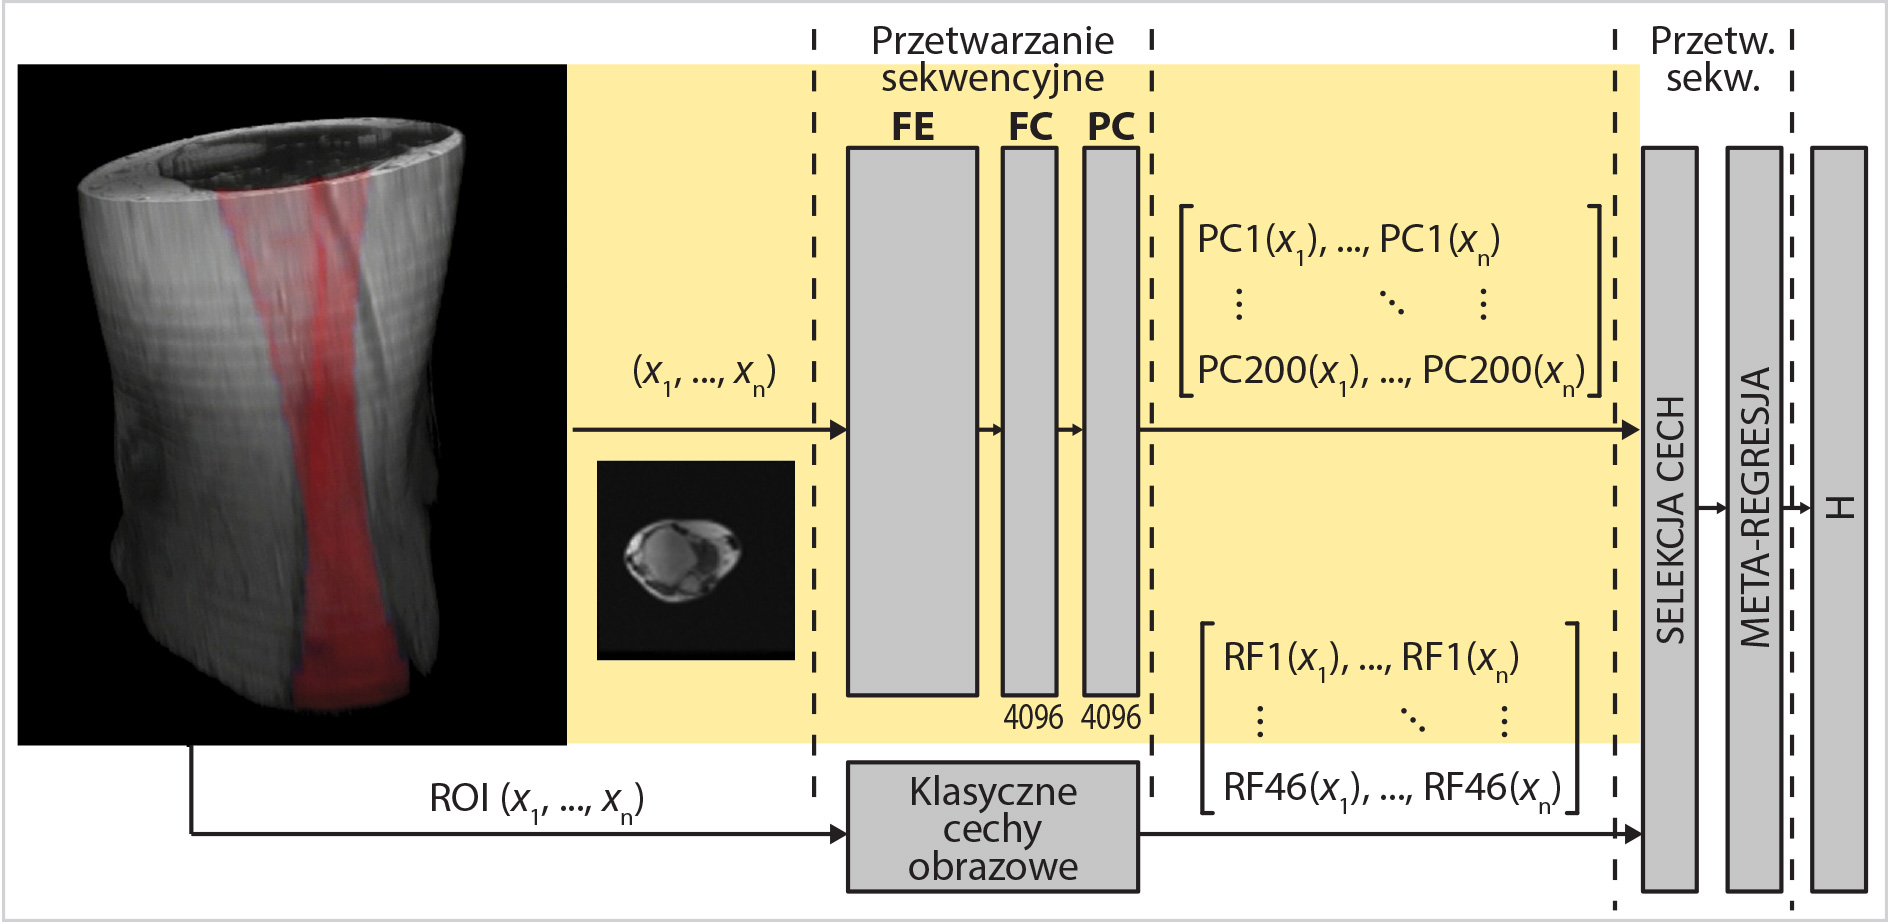
\includegraphics[width=\textwidth]{figures/net.jpg}
	\caption{Schemat automatycznej metody oceny pojedynczego parametru radiologicznego opisującego proces gojenia się ścięgna Achillesa.} \label{fig:net}
\end{figure}

Danymi wejściowymi jest trójwymiarowy obraz obszaru podudzia otrzymany \linebreak w badaniu RM. Badanie dzielone jest na $n$ obrazów będących przekrojami poprzecznymi względem osi długiej ścięgna. Z każdego przekroju dwojako ekstrahowane \linebreak są zestawy cech. Po pierwsze, wykorzystywany jest ekstraktor cech będący złożeniem warstw konwolucyjnych i jednej warstwy gęstej wytrenowanej sieci neuronowej na wyjściu (po redukcji z wykorzystaniem metody analizy czynników głównych) generującej 200 wartości. Po drugie, dla obszaru ścięgna widocznego na każdym z przekrojów, wyliczane są cechy statystyczne i teksturalne, których łączna liczba wynosi 46. Spośród tak utworzonego zestawu 246 wartości, dla każdego z 6-ciu radiologicznych parametrów, wybierane są z wykorzystaniem metody LASSO optymalne podzbiory o liczebności mniejszej niż 20. Podzbiory są kolejno procesowane z wykorzystaniem regresji opartej o algorytm wektorów nośnych, której wyniki dla poszczególnych przekrojów łączone są z wykorzystaniem średniej trymowanej odrzucającej rezultaty skrajne i generującej pojedynczą wartość parametru dla całego badania 3D RM.   


{\let\clearpage\relax\chapter*{Charakterystyka i wyniki przeprowadzonych badań}}
\addcontentsline{toc}{chapter}{Charakterystyka i wyniki przeprowadzonych badań}

Eksperymenty podzielono na dwa etapy. W pierwszym zrealizowano zagadnienia związane z doborem parametrów komponentów nowej metody i oceną jej skuteczności działania. W drugim porównano skuteczność nowej metody z innymi koncepcjami oceny gojenia ścięgna Achillesa. 

W ramach pierwszego etapu wyłoniono, spośród 10-ciu modalności RM analizowanych w pracy, jedną sekwencję będącą najlepszym kandydatem na dane wejściowe. W tym celu zrealizowano zarówno badania związane z analizą wizualną jak i testami ilościowymi. Jednocześnie zbadano, iż dodawanie kolejnych sekwencji nie miało istotnie statycznego wpływu na polepszenie jakości predykcji wartości parametrów radiologicznych, a skutkowało wydłużeniem czasu badania pacjenta. 

W ramach badań nad doborem parametrów nowej metody zrealizowano następujące działania:
\begin{enumerate}
	\item Zoptymalizowano parametry ekstraktora cech poprzez zadanie treningu z celem binarnego podziału obrazów pacjentów na zdrowe i chore ścięgna. Przetestowano 3 architektury sieci neuronowych i na podstawie analizy ich dokładności klasyfikacji oraz czasu treningu wybrano sieć AlexNet. Takie podejście umożliwiło zakodowanie w ekstraktorze jąder konwolucji umożliwiających ekstrakcję charakterystycznych cech dla tkanki zdrowej i patologicznej oraz finalne pogrupowanie ich w wektor o wymiarze 4096.
	\item Przeprowadzono analizę czynników głównych i wykonano redukcję przestrzeni z 4096 parametrów do 200-tu z zachowaniem blisko 99\% poziomu wariancji.
	\item Zrealizowano fuzję i selekcję cech pochodzących z ekstraktora z 46-cioma cechami wybranymi na podstawie analizy literatury, ekstrahowanymi z obszaru ścięgna. W tym celu wykorzystano własność metody LASSO związaną z zerowaniem się współczynników mających marginalny wpływ na ostateczny wynik zadania.
	\item Określono optymalne podzbiory predyktorów dla każdego z 6-ciu parametrów radiologicznych stosując kryterium selekcji współczynników jako najlepszą korelację ocen radiologa z krzywymi gojenia się generowanymi przez automat.
	\item Stosując metodę generalizacji stosów (ang. \textit{stacking}) wytrenowano oraz porównano szereg meta-regresorów: maszynę wektorów nośnych, wielowarstwowy perceptron, drzewa losowe jak i regresję liniową oraz nieliniową. W wyniku badania wybrano algorytm bazujący na wektorach nośnych (SVR), który dla każdego przekroju badania 3D oblicza ocenę z zakresu 0--7 dla zadanego parametru radiologicznego.
	\item Finalnie zrealizowano metodę oceny badania 3D stosując średnią z odrzuceniem wartości skrajnych wyników dla poszczególnych przekrojów.
\end{enumerate}

Opracowaną metodę (SVR) zwalidowano z wykorzystaniem zbioru testowego tj. 4-ech pacjentów (40 badań). Do oceny wykorzystano miary średniego błędu absolutnego (MAE) z informacją na temat błędu średniej, maksymalnego błędu absolutnego (MAX-AE) i średniej korelacji obliczonej z wykorzystaniem transformacji z-Fishera (Corr). Ocenę wykonano dla wszystkich sześciu parametrów radiologicznych:

\begin{enumerate}[noitemsep,nolistsep]
	\item Uszkodzenia śródścięgniste (SCT od ang. \textit{Structural Changes within Tendon}).
	\item Pogrubienie ścięgna (TT od ang. \textit{Tendon Thickening}).
	\item Ostrość granic ścięgna (STE od ang. \textit{Sharpness of the Tendon Edges}).
	\item Obrzęk ścięgna (TE od ang. \textit{Tendon Edema}).
	\item Jednorodność ścięgna (TU od ang. \textit{Tendon Uniformity}).
	\item Obrzęk tkanek (TisE od ang. \textit{Tissue Edema}).
\end{enumerate}

Nową metodę porównano również z dwiema innymi propozycjami oceny gojenia się ścięgna opracowanymi w grupie pod kierownictwem autora tej rozprawy, który odpowiadał za sformułowanie założeń eksperymentów i ich analizę, oraz z metodą bazującą na testach biomechanicznych realizowaną u partnera klinicznego. W dwóch pierwszych podejściach trening przeprowadzono w koncepcji end-to-end tak, aby sieci modelowały \textit{explicite} ocenę radiologa wykorzystując (1) poetykietowane obrazy RM, (2) poetykietowane obrazy ultrasonografii (USG).

Wśród najbardziej interesujących wyników uzyskanych w pracy należy wyróżnić:

\begin{enumerate}
	\item Wybór sekwencji jako danych wejściowych T2$^\ast$ GRE TE\_MIN, w której obraz ścięgna bardzo dobrze różnicuje etapy gojenia się. Taki proces, ze szczególnym pokazaniem różnic w poziomach jasności w obszarze ścięgna, widoczny jest \linebreak na rysunku poniżej.
	\begin{figure}[h!]
		\raggedleft 
		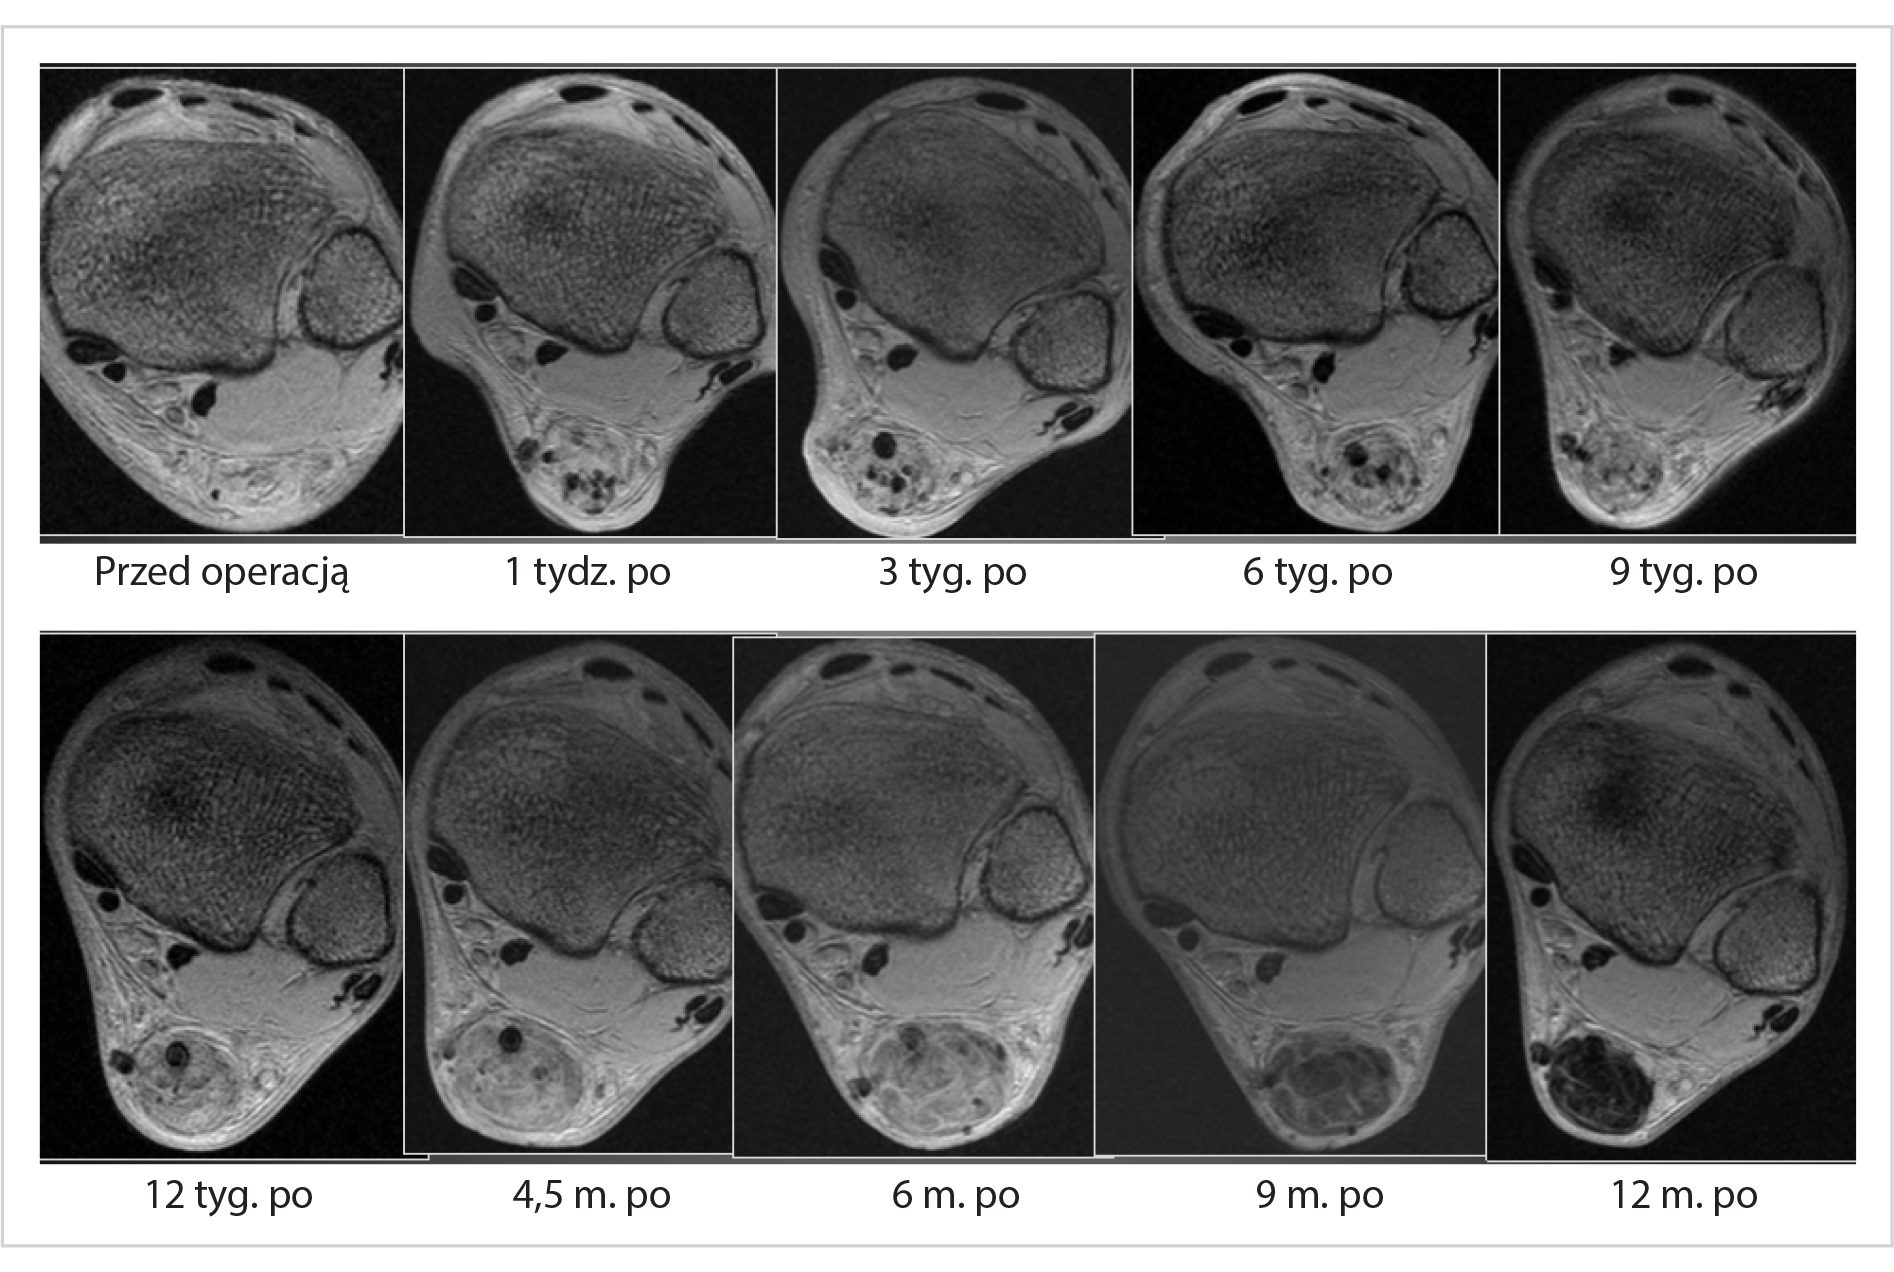
\includegraphics[width=0.93\textwidth]{figures/T2gremin.jpg}
		\captionsetup{margin={1cm,0cm}, font = footnotesize}\caption{Proces gojenia się ścięgna Achillesa widoczny w obrazach zrekonstruowanych na podstawie danych z sekwencji T2$^\ast$ GRE TE\_MIN.}\label{fig:T2comp}
	\end{figure}
	
	Skrócenie protokołu badania z 10-ciu do jednej modalności przełożyło się \linebreak na skrócenie czasu potrzebnego na akwizycję danych od pacjenta. W przypadku protokołu stosowanego w projekcie START jest to oszczędność około 50 min. Natomiast w przypadku standardowego protokołu, rutynowo stosowanego w klinikach oszczędność to około 15 min. biorąc pod uwagę obecny stan techniki. 
	\item Uzyskanie oceny automatu porównywalnej z poziomem oceny radiologa (np. MAE w zakresie 0,56--1,05 dla 40-tu testowych badań). Szczegóły w Tabeli \ref{tab:trainset}. Biorąc pod uwagę również błąd w ocenie radiologa, czyli niedoskonałość wzorca odniesienia, spowodowany np. zmęczeniem, niedoborem czasu itp. uzyskane wyniki są wysoce satysfakcjonujące.
		\vspace{0.5 cm}
	\begin{table}[h!]		
		\captionsetup{margin={1cm,0cm}, font = footnotesize}\caption{Wyniki oceny procesu gojenia z wykorzystaniem proponowanej metody.}
		\vspace{-0.5 cm}
		\tiny
		\begin{center}
			\begin{tabular}{lc||c|c|c|c|c|c}
				\textbf{Model} & & \textbf{SCT} & \textbf{TT} & \textbf{STE} & \textbf{TE} & \textbf{TU} & \textbf{TisE}\\ 				
				\hline \hline
				\multirow{3}{*}{SVR}
				& MAE & 1,05$\pm0,06$ & $0,56\pm0,03$ & $0,75\pm0,04$ & $0,91\pm0,05$ & $0,91\pm0,04$ & 0,94$\pm0,05$\\
				& MAX-AE & 2,62 & 1,82 & 1,92 & 2,54 & 2,01 & 2,38 \\
				& Corr   & 0,85 & 0,85 & 0,31 & 0,72 & 0,65 & 0,80 \\
				\hline
			\end{tabular}
		\end{center}
		\label{tab:trainset}
	\end{table}	
\vspace{-0.5 cm}
	\item Zrealizowanie warstwy prezentacji z oceną krzywych gojenia. Przykład takich krzywych znajduje się na poniższym rysunku.
	 \begin{figure}[h!]
	 	\raggedleft
	 	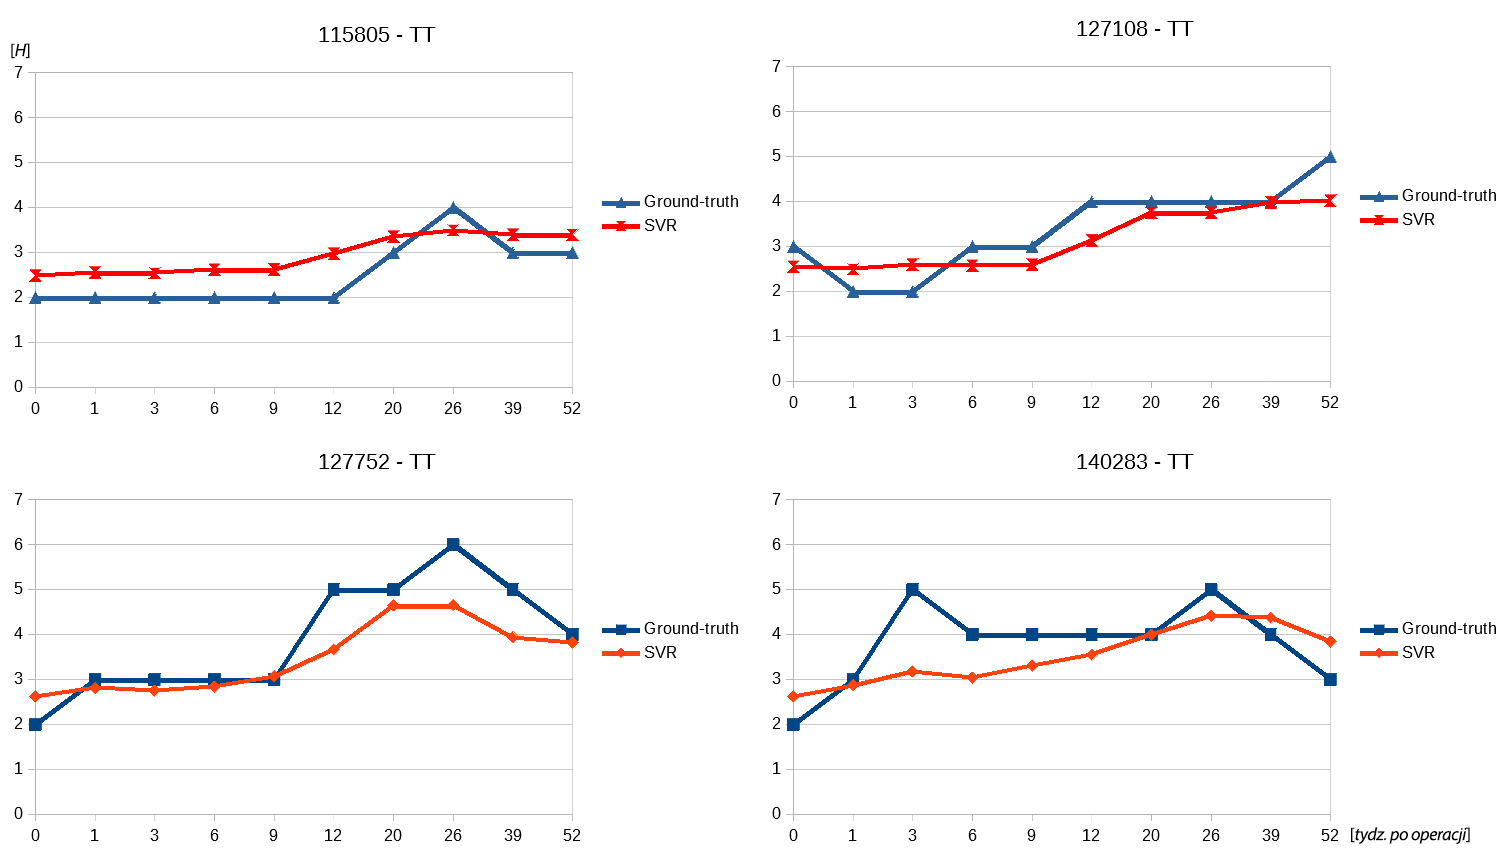
\includegraphics[width=0.93\textwidth]{figures/TT.png}
	 	\captionsetup{margin={1cm,0cm}, font = footnotesize}\caption{Ocena parametru TT.}\label{fig:TT}
	 \end{figure}
 
 W pracy ponadto zaproponowano przykładowy raport, który mógłby być generowany dla każdego z pacjentów oraz ocenę holistyczną będącą wynikiem analizy czynników głównych dla zbioru parametrów radiologicznych. Całość prac była nacelowana na ułatwienie przepływu informacji między osobami najbardziej zaangażowanymi w proces rehabilitacji pacjenta tj. radiologiem, ortopedą i fizjoterapeutą.
 \item Porównanie z innym podejściem tj. modelującym bezpośrednio ocenę radiologa (zob. Tab. \ref{tab:end-to-end_testset}). W zestawieniu z alternatywną metodą analizy obrazów RM, wykazano przewagę zaproponowanego podejścia w kontekście oceny trendów gojenia się i uzyskiwanych średnich błędów, a dokładniej uzyskano istotnie statystycznie lepsze rezultaty dla 4 z 6-ciu parametrów, a istotne pogorszenie tylko w jednym.
 \vspace{0.5cm}
 %\renewcommand{\arraystretch}{1.2}
 \begin{table}[h!]
 	\captionsetup{margin={1cm,0cm}, font = footnotesize}\caption{Porównanie wyników wnioskowania z wykorzystaniem zbioru testowego dla metody proponowanej tj. SVR oraz metody wyszkolonej w paradygmacie end-to-end (Inception-v3$_{e}$). Pogrubieniem oznaczono najlepsze rezultaty, a kolorem czerwonym istotne statystycznie różnice w liczonych średnich ($p$ $<$ 0,05).}
 	\vspace{-0.5cm}
 	\tiny
 	\begin{center}
 		\hspace*{2em}\begin{tabular}{lc||c|c|c|c|c|c}
 			\textbf{Model} & & \textbf{SCT} & \textbf{TT} & \textbf{STE} & \textbf{TE} & \textbf{TU} & \textbf{TisE}\\ \hline \hline
 			Inception-v3$_{e}$ & MAE & 1,12$\pm{0,08}$ & 0,80$\pm{0,04}$ & 1,40$\pm{0,07}$ & \textbf{0,89}$\pm{0,05}$ & 1,08$\pm{0,04}$ & \textcolor{red}{\textbf{0,69}}$\pm{0,07}$ \\
 			& MAX-AE & \textbf{2,14} & \textbf{1,01} & 2,13 & \textbf{1,18} & \textbf{1,44} & \textbf{0,78} \\
 			& Corr & 0,82 & 0,77 & 0,05 & 0,59 & 0,52 & 0,77 \\ \hline
 			SVR & MAE & \textbf{1,05}$\pm0,06$ & \textcolor{red}{\textbf{0,56}}$\pm0,03$ & \textcolor{red}{\textbf{0,75}}$\pm0,04$ & 0,91$\pm0,05$ & \textcolor{red}{\textbf{0,91}}$\pm0,04$ & $0,94\pm0,05$\\
 			& MAX-AE & 2,62 & 1,82 & \textbf{1,92} & 2,54 & 2,01 & 2,38 \\
 			& Corr & \textbf{0,85} & \textbf{0,85} & \textcolor{red}{\textbf{0,31}} & \textcolor{red}{\textbf{0,72}} & \textcolor{red}{\textbf{0,65}} & \textbf{0,80} 
 		\end{tabular}
 	\end{center}
 	\label{tab:end-to-end_testset}
 \end{table}
\vspace{-1cm}
 %\renewcommand{\arraystretch}{1}
 \item Porównanie z podejściem bazującym na ocenie procesu gojenia widocznym \linebreak na zdjęciach z ultrasonografii (zob. Tab. \ref{tab:USGvsRM-cross-validation}). W tym przypadku wykazano możliwość synergii podejść, bazując na większej izotropowości danych USG i dobrych wynikach oceny parametrów widocznych w płaszczyźnie strzałkowej.
 %\renewcommand{\arraystretch}{1.2}
 \vspace{0.3cm}
 \begin{table}[h!]
 	\tiny
 	\setlength{\tabcolsep}{1pt}
 	\captionsetup{margin={1cm,0cm}, font = footnotesize}\caption{Porównanie wyników oceny automatycznej, bazującej na danych USG i RM, dla pacjentów ze zbioru testowego. Pogrubieniem oznaczono najlepsze wyniki. Kolorem czerwonym oznaczono poprawę w stosunku do kolejnego wyniku istotną statystycznie z $p$$<$0,05.}
 	\label{tab:USGvsRM-cross-validation}
 	\vspace{-0.3cm}
 	\hspace*{3.5em}\begin{tabular}{lc||c|c|c|c|c|c}
 		%\hline
 		& & \multicolumn{6}{c}{\textbf{USG -- p. strzałkowy}} \\
 		\textbf{Model} & & \textbf{SCT} & \textbf{TT} & \textbf{STE} & \textbf{TE} & \textbf{TU} & \textbf{TisE} \\ \hline \hline
 		Inception-v3$_{eus}$ & MAE & \textbf{0,81}$\pm$0,19 & 0,63$\pm$0,03 & \textbf{0,56}$\pm$0,09 & 0,85$\pm$0,10 & 0,54$\pm$0,02 & 0,87$\pm$0,14 \\
 		& MAX-AE & 1,59 & 1,79 & 1,7 & \textbf{1,25} & \textbf{1,38} & 1,69 \\
 		& Corr & 0,80 & 0,77 & 0,31 & 0,52 & \textbf{0,69} & 0,62 \\ \hline
 		ResNet-50$_{eus}$ & MAE & 0,88$\pm$0,16 & 0,65$\pm$0,07 & 0,66$\pm$0,04 & 0,83$\pm$0,12 & 0,75$\pm$0,06 & 0,93$\pm$0,11 \\
 		& MAX-AE & \textbf{1,49} & \textbf{1,26} & 1,74 & 1,48 & 1,78 & 1,71 \\
 		& Corr & 0,60 & 0,55 & 0,25 & 0,55 & 0,34 & 0,56 \\
 		\hline \hline
 		& & \multicolumn{6}{c}{\textbf{USG -- p. poprzeczny}} \\
 		
 		Inception-v3$_{euo}$ & MAE & 0,84$\pm$0,27 & 0,75$\pm$0,7 & 0,58$\pm$0,05 & 0,83$\pm$0,05 & \textcolor{red}{\textbf{0,53}}$\pm$0,08 & \textbf{0,83}$\pm$0,15 \\
 		& MAX-AE & 2,8 & 1,46 & \textbf{1,51} & 1,27 & 1,63 & 1,65 \\
 		& Corr & 0,69 & 0,68 & \textbf{0,45} & 0,51 & 0,66 & 0,68 \\ \hline
 		ResNet-50$_{euo}$ & MAE & 0,92$\pm$0,18 & 0,76$\pm$0,16 & 0,68$\pm$0,04 & \textbf{0,81}$\pm$0,08 & 0,65$\pm$0,10 & 0,94$\pm$0,05 \\
 		& MAX-AE & 2,01 & 1,56 & 1,61 & 1,69& 1,43 & \textbf{1,58}\\
 		& Corr & 0,55 & 0,57 & 0,35 & 0,44 & 0,39 & 0,61 \\ \hline \hline
 		& & \multicolumn{6}{c}{\textbf{Rezonans magnetyczny}} \\
 		
 		SVR & MAE & $1,05\pm0,06$ & \textbf{0,56}$\pm0,03$ & $0,75\pm0,04$ & $0,91\pm0,05$ & $0,91\pm0,04$ & $0,94\pm0,05$\\
 		& MAX-AE & 2,62 & 1,82 & 1,92 & 2,54 & 2,01 & 2,38 \\
 		& Corr   & \textbf{0,85} & \textbf{0,85} & 0,31 & \textcolor{red}{\textbf{0,72}} & 0,65 & \textcolor{red}{\textbf{0,80}} \\
 		
 	\end{tabular}
 \end{table}
 %\renewcommand{\arraystretch}{1}
 \vspace{-1cm}
 \item Zrealizowano porównanie oceny holistycznej (pierwszy czynnik główny z wartości parametrów radiologicznych) z testami ATRS i deficytami sił mięśniowych, dla których w pracy z wykorzystaniem analizy czynników głównych zaproponowano 4 zmienne (WW, WZ, ZW, ZZ) związane z pozycją kończyny dolnej. Szczegółowe wyniki znajdują się w Tab. \ref{tab:bioATRSvspredGT}. Badania biomechaniczne były realizowane w ramach protokołu monitorowania rehabilitacji pacjentów opracowanego w klinice Carolina Medical Center. Porównania ilościowe przedstawione w pracy potwierdziły znane w literaturze fakty (np. wskazania radiologa słabo korelują z wynikami badań biomechanicznych oraz ATRS) jak \linebreak i dostarczyły wskazówek odnośnie możliwych nowych obszarów badań np. stworzenia nowatorskiego, komplementarnego testu bazującego na fuzji informacji biomechanicznych i z obrazowania medycznego. 
 \vspace{0.5 cm} 
 \begin{table}[h!]
 	\setlength{\tabcolsep}{3pt}
 	\setlength\extrarowheight{2pt}
 	\captionsetup{margin={1cm,0cm}, font = footnotesize}\caption{Korelacja badań biomechanicznych i ATRS z badaniami radiologicznymi ocenionymi automatycznie i przez radiologa. Oznaczone korelacje są istotne z $p$$<$0,05 dla $N$=30.}
 	\label{tab:bioATRSvspredGT}
 	\footnotesize
 	\hspace*{3em}\begin{tabular}{c|c|c}
 		&ocena automatyczna&ocena radiologa \\
 		\hline \hline
 		WW&0,1197&0,0706\\
 		\hline
 		WZ&0,1576&0,1931\\
 		\hline
 		ZW&0,3429&0,3092\\
 		\hline
 		ZZ&0,3100&0,2996\\
 		\hline
 		ATRS&\textbf{0,3854}&0,2088\\		
 	\end{tabular}
 \end{table}
\end{enumerate}
\vspace{-1 cm} 
{\let\clearpage\relax\chapter*{Wnioski końcowe}}
\addcontentsline{toc}{chapter}{Wnioski końcowe}

W ramach pracy osiągnięto wszystkie założone cele jak i potwierdzono postawioną hipotezę dokumentując utylitarność głębokich sieci neuronowych w kontekście oceny ścięgna Achillesa widocznego w badaniu RM. Zrealizowane badania zostały pozytywnie ocenione przez panel ekspertów Nardowego Centrum Badań i Rozwoju z rekomendacją do ich komercjalizacji. Przedstawione rozwiązanie może być podstawą do budowy narzędzi komputerowo wspomaganej radiologii, w szczególności w zakresie bieżących potrzeb tj. przyspieszenia generowania raportów, polepszenia personalizacji diagnostyki i poprawy jej jakość.

Wstępne szacunki przedstawione w pracy, bazujące na liczbie wykonywanych rocznie opisów badań RM ścięgna Achillesa w USA i Europie Zachodniej wskazują, że poprzez wspomaganie generowania raportów w zakresie przedmiotowego badania, sumarycznie, możliwa jest oszczędność do 83 tys. godzin pracy radiologów rocznie. Opracowane metody mogą również wspomóc wczesną detekcję zmian strukturalnych ścięgna i zredukować finalną liczbę zerwań. Certyfikowane narzędzie zaprojektowane na bazie przedstawionych algorytmów, żywotnie wpisałoby się również w ideę poprawy jakości diagnostyki, umożliwiając gromadzenie ustrukturyzowanych danych, porównań między pacjentami i holistycznego wnioskowania będącego katalizatorem innowacji. Autor ma nadzieję na realizację kolejnych etapów w ramach działań związanych z założoną w Styczniu 2020 r. spółką spin-off Uniwersytetu Warszawskiego.

         

\end{document}